\chapter{Ausgangslage und Zielstellung}\label{cha:Ausgangslage und Zielstellung}

Die in diesem Bericht dokumentierte Auslegung beschäftigt sich mit dem Tragflügel des studentischen AUVSI Flugzeugs, welches im Labor für Systemtechnik entwickelt wurde. Die vorangegangenen Flugzeuggenerationen und das Reglement des Wettbewerbs bilden die Ausgangslage für die Weiterentwicklung.

\section{Historie des AUVSI SUAS-Wettbewerbs}
Seit 2002 findet jährlich der AUVSI (Association for Unmanned Vehicle Systems International) SUAS (Student Unmanned Aerial Systems Competition)-Wettbewerb in den USA statt.

Hieran hat das studentische Hochschulteam in den Jahren 2015 und 2016 erfolgreich teilgenommen. Bereits im Jahr 2014 gab es die ersten Anstrengungen eine für diesen Wettbewerb passende Entwicklung einer Flugplattform. Leider war dies zum gegebenen Zeitpunkt noch nicht zum Erfolg. Detaillierte Informationen hierzu können der Diplomarbeit von Herrn Dipl. Ing. Fabian Meilinger entnommen werden \cite{Meiling}.

Die meisten Anforderungen an die Flugplattform ergeben sich aus dem Reglement des genannten studentischen Wettbewerbs. 

\clearpage

\section{Das Flugzeug des AUVSI SUAS Teams}

Aufbauend auf den ersten Erfahrungen in der Saison 2014 folgt der konzeptionelle Aufbau des Flugzeugs einem modularen Konzept. Dies ermöglichte mit definieren Schnittstellen zwischen den Baugruppen eine getrennte Weiterentwicklung der jeweiligen Einzelkomponenten. Hieraus entstanden zum Beispiel 2015 Variationen für die Forschungsmission im Regenwald Ecuadors, bei der eine deutlich voluminösere Nutzlast mitgeführt werden sollte. \cite{Niclas}.

\begin{figure}[H]
\centering
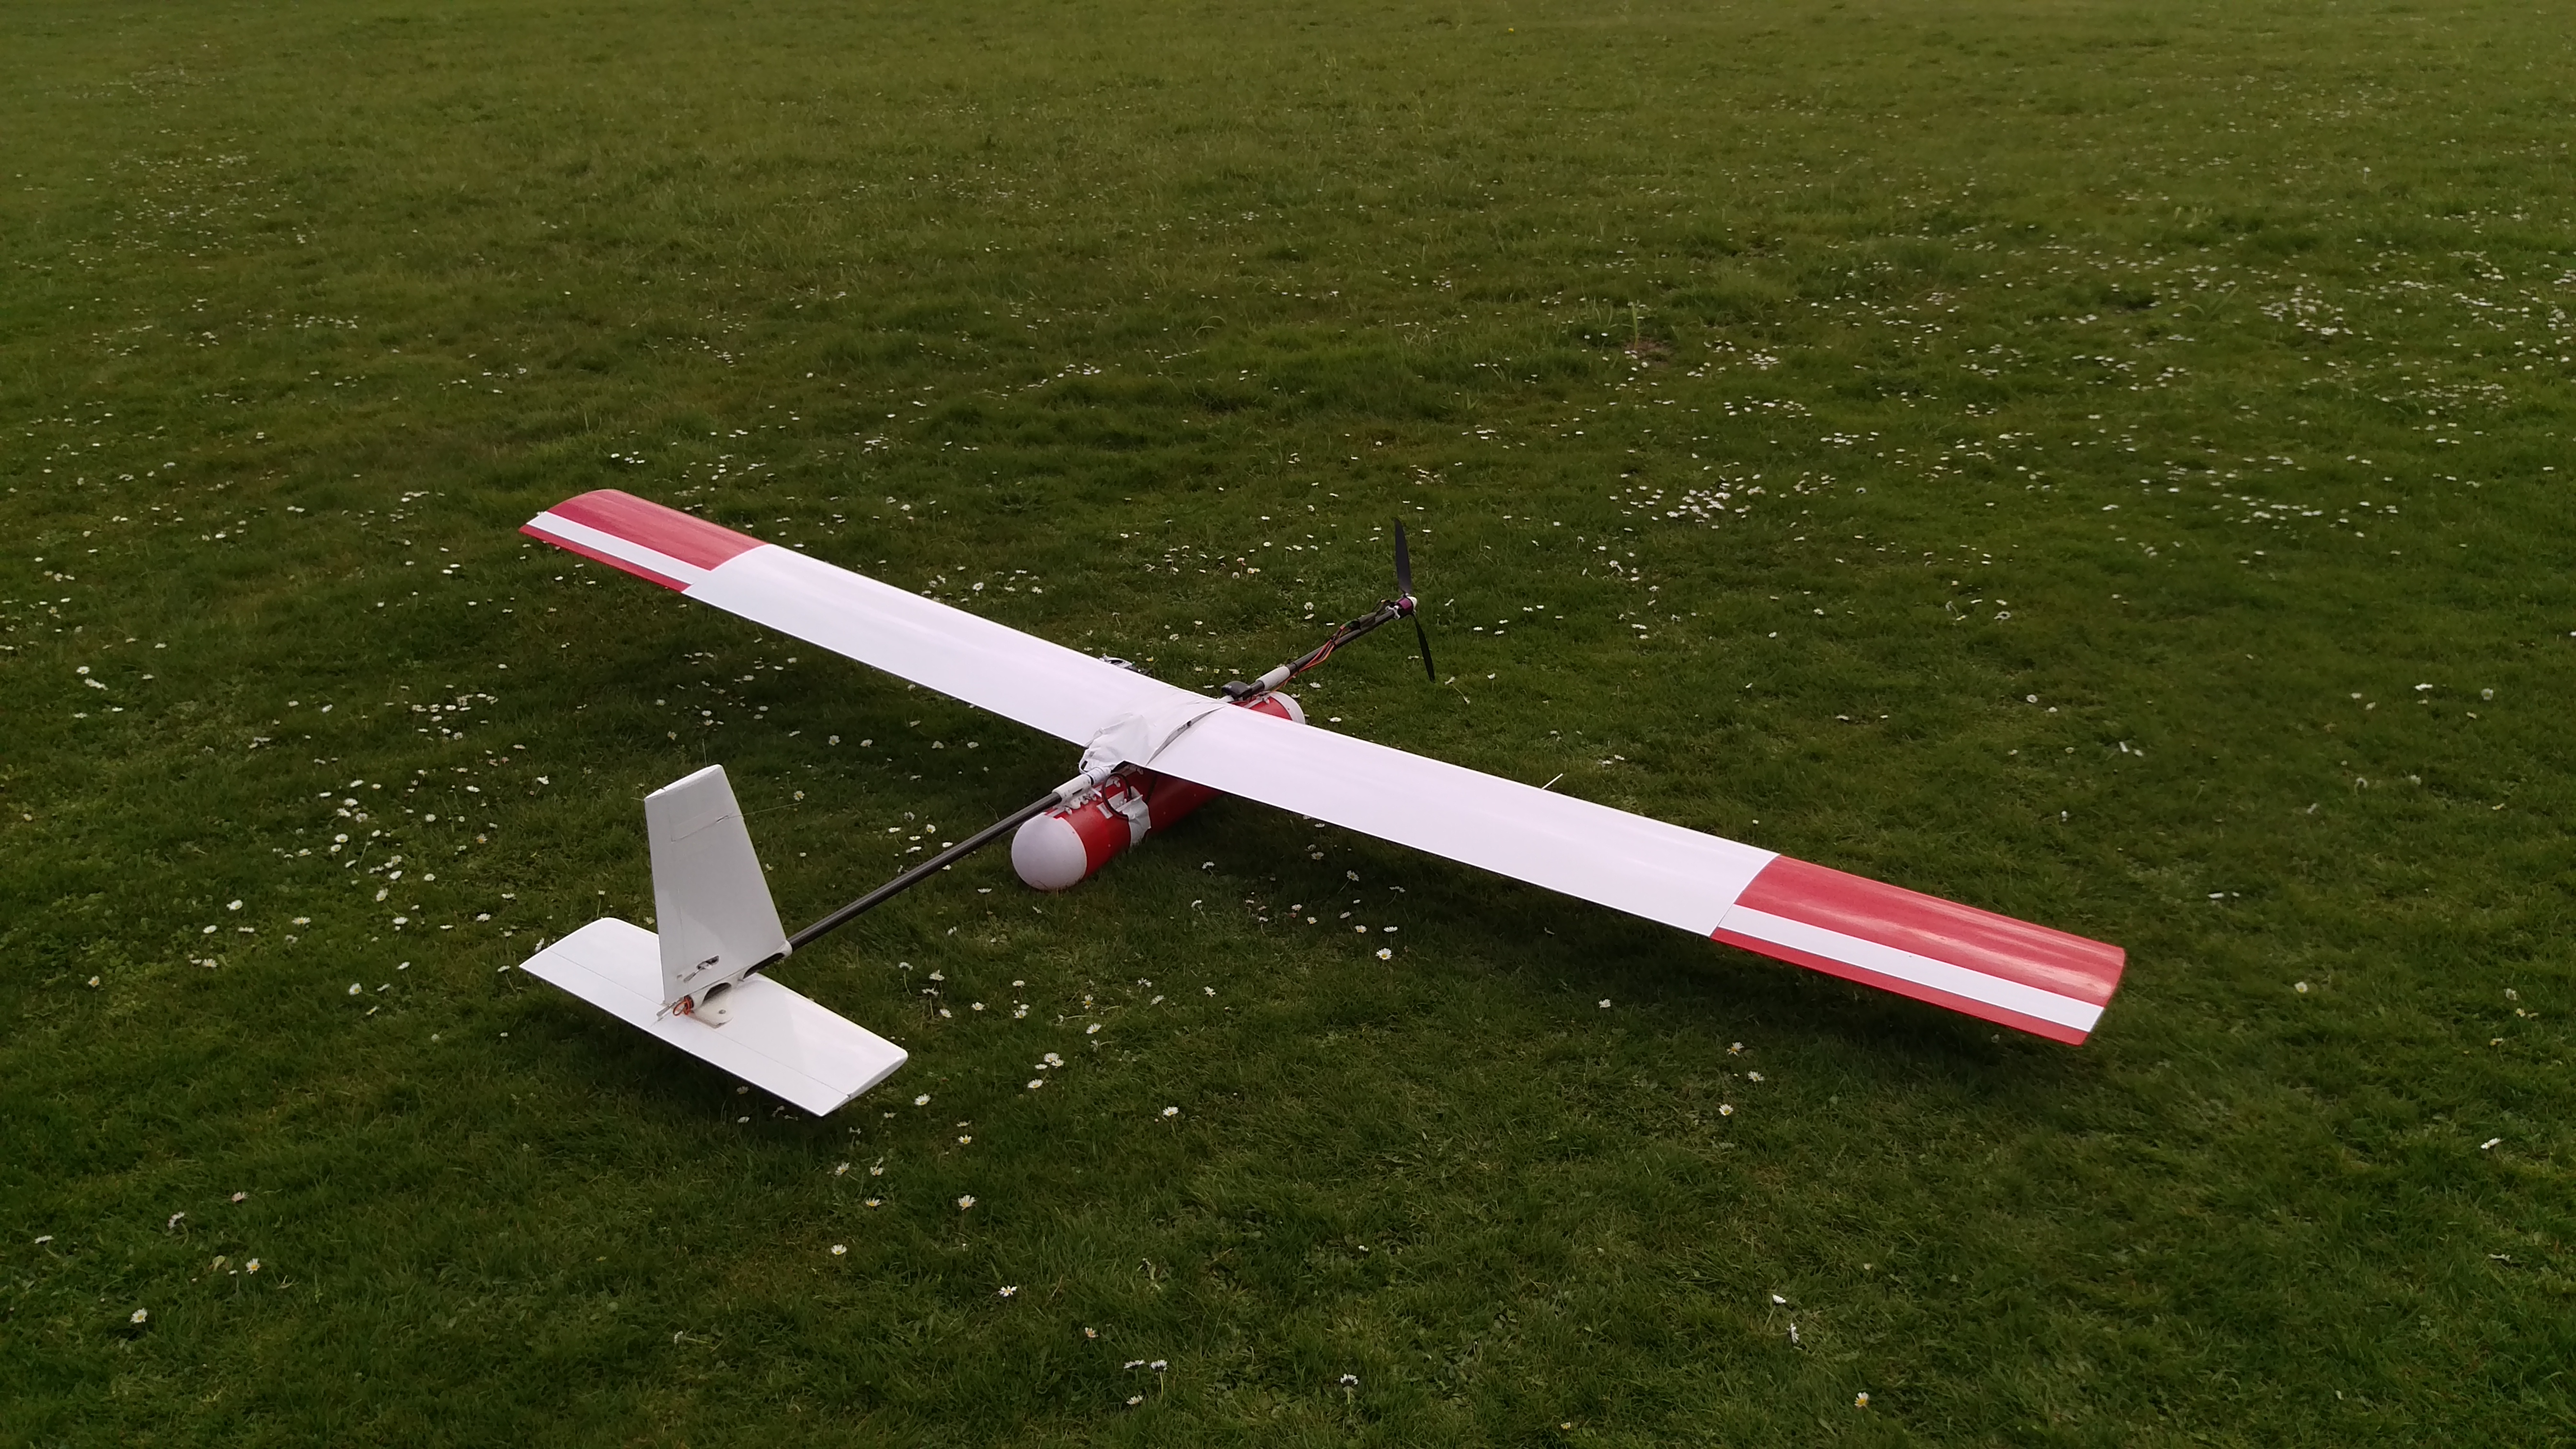
\includegraphics[width=0.9\textwidth]{bilder/Fotos/AUVSI_2015.jpg} 
\caption{Das AUVSI 2015 Modell im Einsatzzustand am Testflugplatz} 
\label{fig:Das AUVSI 2015 Modell in Einsatzzustand am Testflugplatz}
\end{figure}

Im Bild \ref{fig:Das AUVSI 2015 Modell in Einsatzzustand am Testflugplatz} ist der Gesamtaufbau des Flugzeugs zu sehen. Bisher sind der Einsatz von rechteckigen Tragflächen und Leitwerken sowie CFK-Rohren als Ausleger für Heck und Motorträger charakteristisch. Unter dem zentralen Rumpfrohr ist der zylinderförmige Nutzlastbehälter montiert.


\clearpage


\section{Bisherige Flügelbauweise}

Die bisherigen Tragflügel sowie einige Leitwerksflächen wurden in der, in Modellbaukreisen, als \glqq Styro-Abachi\grqq{} bekannte Bauweise ausgeführt. Die Tragflächen des AUVSI-UAV's sind bisher von einem Kern aus Polystyrol gefertigt worden. In einem ersten Schritt wird mit Hilfe einer 4-Achs CNC Heißdrahtschneidemaschine die gewählte Profilform (Clark-Y) aus einem Styroporkern geschnitten. In diesen Rohling werden anschließend Aussparungen für die Kabelschächte und die Servomotoren der Rudermaschinen eingebracht. Auf Ober- und Unterseite der Fläche wird Abachi Furnier mit einer Schichtstärke von 0,6 mm verklebt. Dabei wird während der Aushärtephase des Klebstoffs ein Vakuumsack eingesetzt, um die Festigkeit der Klebeverbindung zu steigern.
Auf beide Enden werden Endrippen aus 3 mm starkem Ceibasperrholz aufgebracht. Die Kraftübertragung in die anschließenden Segmente wird durch, in die Polystyrolblöcke eingeklebte, CFK-Rohre realisiert. Daran anschließend erfolgt das Auskasten und Anschlagen der Ruderflächen.
Abschließend wird die Fläche mit heißklebender Kunststofffolie mit Hilfe eines Bügeleisens überzogen zur Steigerung der Resistenz  gegen Umwelteinflüsse.

Bei dieser Bauweise soll der Großteil der Zugspannungen vom aufgebrachten Abachi Furnier in Faserrichtung aufgenommen werden. Der Polystyrolkern soll hingegen die Übertragung der Schubspannungen zwischen Ober- und Unterseite der Tragfläche gewährleisten und nimmt zusätzlich entstehenden Druck quer zur Oberfläche auf. Als problematischer Parameter, der die Biegefestigkeit der Gesamtstruktur erheblich reduziert, hat sich die Festigkeit der Klebeverbindung zwischen oberer Furnierlage (Druck) und dem Polystyrolkern herauskristallisiert. Ein Versagen der Verklebung führt zum Abschälen des Furniers, was Druckbeulen der oberseitigen Furnierlage nach sich zieht. Dies führt zu einem Stabilitätsversagen.

Insgesamt hat sich diese Bauweise als sehr robust erwiesen, sie  hat eine ausreichende Stabilität in allen Flugsituationen nachgewiesen.
Die Formabweichungen von der gewählten Profilform sind vergleichsweise gering. Dies setzt allerdings den Einsatz von korrekt gefertigten Werkzeugen während des Vakuumverfahrens voraus und eine fehlerfreie Durchführung der oben genannten Verfahrensschritte.  

Nachteilig ist das vergleichsweise hohe Gewicht von \SI[per-mode=symbol]{2,145}{\kilogram\per\meter\squared} [AUVSI/Ecuador 2015].
Zusätzlich wird für die Fertigung ein einfacher Werkzeugbau benötigt und es ergeben sich zahlreiche Arbeitsschritte, die zum Teil hohes handwerkliches Geschick erfordern. Damit variiert die Qualität der Ergebnisse deutlich je nach Erfahrung und Sorgfalt des fertigenden Personals. Besonders Fehler beim Vakuumverkleben der Furnierschichten können das gesamte Tragflächensegment unbrauchbar machen. 

Bisher sind weder eine Vorauslegung noch eine Dimensionierung der Struktur für die erwarteten Lasten durchgeführt worden.

Erfahrungen aus Belastungs- und Überlastungsversuchen mit früheren Tragflächen dieser Bauweise lassen erwarten, dass die bisherige Struktur bedeutend überdimensioniert ist mit negativen Auswirkungen auf die erzielbaren Flugleistungen. 

\clearpage

\section{Verbesserungsziele}

Ziele dieser Arbeit sind Verbesserungen der jetzigen Bauform in folgenden Bereichen:
\begin{itemize}
    \item Nachweis der Festigkeit der Fläche bei bekannten Sicherheiten und Lastgrenzen
    \item Reduzierung des Flächengewichts durch bessere Ausnutzung der Materialkennwerte
    \item Reduzierung des Anteils an anspruchsvoller Handarbeit und Steigerung des Anteils mechanisierter und werkzeugbasierter Fertigung
    \item Einsatz einer möglichst profiltreuen Bauweise bis zu mindestens 25\% der Flächentiefe.
    \label{lst:Verbesserungsziele}
\end{itemize}


\section{Optimierungsgrenzen durch den Einsatz}

Der Optimierung des Flügels auf die in \ref{lst:Verbesserungsziele} genannten Ziele sind durch den praktischen Einsatz einige Grenzen gesetzt.
Im Folgenden sollen Situationen beschrieben werden, die im Alltagseinsatz des Fluggeräts auftreten und die zu Belastungen der Struktur führen, die weit über die im statischen Flugzustand  liegen können. 

Mit dem Fluggerät wird im Normalfall von einer kurzen Rampe ein Flitschenstart durchgeführt. Dabei wird das UAV durch ein Gummiseil bis knapp über die festgelegt Mindestfluggeschwindigkeit beschleunigt. Dadurch entstehen kurzzeitige Lastvielfache von bis zu 3,5 g in Flugrichtung.
Auch ein Hochstart wurde für spezielle Einsätze in Erwägung gezogen, in denen der Energieverbrauch zum Erreichen der Missionshöhe einen zu hohen Anteil an der Gesamtflugaufgabe hätte. 
Dabei muss die Tragfläche kurzzeitig deutlich höhere Belastungen durch  Auftriebskräfte als beim statischen Reiseflug aushalten. 

Zusätzlich treten im Alltagseinsatz eine Reihe von atypischen Belastungen auf. So werden die Tragflächen beispielsweise in Transportkisten befördert, beim Aus- und Einladen sowie bei der Montage durch Handkräfte werden diese auf Druck beansprucht. Deshalb bedarf es entweder einer ausreichenden Druckfestigkeit oder einfacher Reparaturmethoden, um die entstandenen Beschädigungen durch unsachgemäße Handhabung zu beseitigen. 
